% Diagrama a bloques de la app de la Práctica 3 (Qt 6, Android) — pdflatex diagrama-bloques-p3.tex
\documentclass[border=8pt]{standalone}
\usepackage[utf8]{inputenc}
\usepackage[T1]{fontenc}
\usepackage{tikz}
\usetikzlibrary{positioning,arrows.meta,fit,backgrounds}
\begin{document}
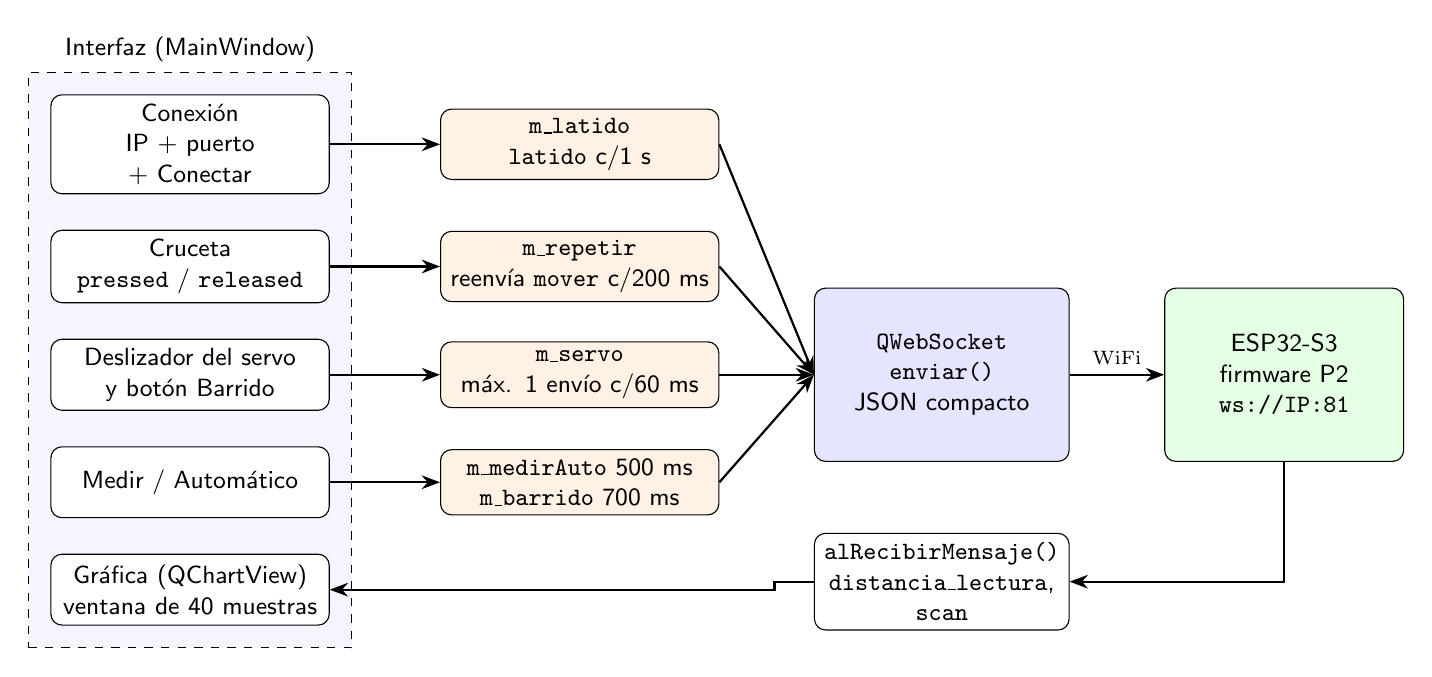
\begin{tikzpicture}[font=\sffamily\small, node distance=0.45cm and 0.9cm,
  b/.style={draw, rounded corners, fill=white, align=center, minimum height=0.9cm, text width=3.3cm},
  t/.style={draw, rounded corners, fill=orange!10, align=center, minimum height=0.8cm, text width=3.3cm},
  fl/.style={-Stealth, thick}]
% Interfaz
\node[b] (con) {Conexión\\IP + puerto + Conectar};
\node[b, below=of con] (cru) {Cruceta\\\texttt{pressed} / \texttt{released}};
\node[b, below=of cru] (ser) {Deslizador del servo\\y botón Barrido};
\node[b, below=of ser] (med) {Medir / Automático};
\node[b, below=of med] (gra) {Gráfica (QChartView)\\ventana de 40 muestras};
\begin{scope}[on background layer]
\node[draw, dashed, fill=blue!4, fit=(con)(gra), inner sep=8pt, label=above:{Interfaz (MainWindow)}] {};
\end{scope}
% Temporizadores
\node[t, right=1.4cm of cru] (rep) {\texttt{m\_repetir}\\reenvía \texttt{mover} c/200 ms};
\node[t, right=1.4cm of ser] (tse) {\texttt{m\_servo}\\máx. 1 envío c/60 ms};
\node[t, right=1.4cm of med] (tme) {\texttt{m\_medirAuto} 500 ms\\\texttt{m\_barrido} 700 ms};
\node[t, right=1.4cm of con] (lat) {\texttt{m\_latido}\\\texttt{latido} c/1 s};
% Socket
\node[b, right=1.2cm of tse, text width=3.0cm, minimum height=2.2cm, fill=blue!10] (ws) {\texttt{QWebSocket}\\\texttt{enviar()}\\JSON compacto};
\node[b, right=1.2cm of ws, text width=2.8cm, minimum height=2.2cm, fill=green!10] (esp) {ESP32-S3\\firmware P2\\\texttt{ws://IP:81}};
\node[b, below=0.9cm of ws, text width=3.0cm] (rx) {\texttt{alRecibirMensaje()}\\\texttt{distancia\_lectura}, \texttt{scan}};
\draw[fl] (con) -- (lat); \draw[fl] (cru) -- (rep); \draw[fl] (ser) -- (tse); \draw[fl] (med) -- (tme);
\foreach \n in {lat,rep,tse,tme} \draw[fl] (\n.east) -- (ws.west);
\draw[fl] (ws.east) -- node[above,font=\scriptsize]{WiFi} (esp.west);
\draw[fl] (esp.south) |- (rx.east);
\draw[fl] (rx.west) -| ([xshift=-0.5cm]rx.west) |- (gra.east);
\end{tikzpicture}
\end{document}
